%%%%%%%%%%%%%%%%%%%%%%%%%%%%%%%%%%%%%%%%%%%%%%%%%%%%%%%%%%%%%%%%%%%%%%%%%%%%%%%%
% oscillation_analysis.tex: Analysis of Neutrino Oscillations:
%%%%%%%%%%%%%%%%%%%%%%%%%%%%%%%%%%%%%%%%%%%%%%%%%%%%%%%%%%%%%%%%%%%%%%%%%%%%%%%%
\chapter{Analysis}
\label{Chapter:analysis}
%%%%%%%%%%%%%%%%%%%%%%%%%%%%%%%%%%%%%%%%%%%%%%%%%%%%%%%%%%%%%%%%%%%%%%%%%%%%%%%%




%%%%%%%%%%%%%%%%%%%%%%%%%%%%%%%%%%%%%%%%%%%%%%%%%%%%%%%%%%%%%%%%%%%%%%%%%%%%%%%%
% Analysis Procedure {{{
%%%%%%%%%%%%%%%%%%%%%%%%%%%%%%%%%%%%%%%%%%%%%%%%%%%%%%%%%%%%%%%%%%%%%%%%%%%%%%%%

\section{Interpretation of Discrepancies}
As was shown in the previous chapter, no simulation model matches the data for the normalized distributions within uncertainty. This disagreement implies that the simulation does not accurately simulate the \bosonpt of the \Z. Due to the similarities in the production of a Z and a W, there is most likely a similar disagreement between the simulated and actual \bosonpt distribution of the W boson. As was mentioned in Chapter \ref{chapter:theory}, the measurement of the W mass is calculated based on the distribution of the leptons \pt distribution, which would be effected by the \bosonpt of the W. As was described in  the same chapter there is currently a tension between the measured and theoretical mass measurement of the W. However, with the high uncertainty of the W mass it is not possible to tell if this tension is real. For this reason it is important to attempt to lower the uncertainty of the measured W mass.  By finding a method to increase the agreement between the theoretical and measured \phistar distribution of the \Z, the uncertainty of the W mass measurement may be lowered allowing to find if the tension between the theoretical and measured W mass is real, and in turn, if there is a flaw with the standard model.

The inconsistency of the \phistar measurement between \POWHEG+\PYTHIAsix and \POWHEG+\PYTHIAeight implies that part of the disagreement between simulation and data may be due to the hadronizer. \PYTHIAeight contains many variables that can be changed that would effect the \phistar distribution. If a set of these variables could be found that fixed the \phistar distribution and that did not reduce the accuracy of the hadronizer for other types of simulations, it would be possible to create a new W boson simulation that was more accurate. This would allow for a W mass measurement to be made more accurately.


%%%%%%%%%%%%%%%%%%%%%%%%%%%%%%%%%%%%%%%%%%%%%%%%%%%%%%%%%%%%%%%%%%%%%%%%%%%%%}}}
%%%%%%%%%%%%%%%%%%%%%%%%%%%%%%%%%%%%%%%%%%%%%%%%%%%%%%%%%%%%%%%%%%%%%%%%%%%%%%%%
% Analysis Result {{{
%%%%%%%%%%%%%%%%%%%%%%%%%%%%%%%%%%%%%%%%%%%%%%%%%%%%%%%%%%%%%%%%%%%%%%%%%%%%%%%%
\section{\PYTHIAsix to \PYTHIAeight comparison}
Due to the large difference between the results of \POWHEG hadronized by \PYTHIAsix compared to \PYTHIAeight, some of the basic changes between parameters used for each of the hadronizers were investigated. These parameters were  $\PtWidth$, which is  the width of the Gaussian used to calculate the $\px$ and $\py$ of the partons used by the hadronizer, and the PDF used by the hadronizer. The test was done by comparing a \POWHEG+\PYTHIAsix sample to four \POWHEG+\PYTHIAeight samples. These \POWHEG+\PYTHIAeight samples were created using different combinations of the default \PYTHIAsix and \PYTHIAeight values of the \PtWidth and PDF.

The variable \PtWidth is of particular interest to the \phistar measurement since a larger \PtWidth results in partons with a larger \pt, which can create a Z with a higher \bosonpt. \PYTHIAeight calculates the value of $\PtWidth$ on a particle-by-particle basis using Eq. \ref{eq:RemWidth}, while \PYTHIAsix keeps \PtWidth constant, with the Z2* tune having $\PtWidth=\SI{2}{GeV}$. A second change between the two was the PDF used by the hadronizers, with the \PYTHIAsix sample using the PDF CTEW6L, and \PYTHIAeight sample using the PDF NNPDF2.3 QCD+QED LO, along with a change in the \alphastrong, with $\alphastrong(\MZ)=0.1180$ and $\alphastrong(\MZ)=0.130$ for \PYTHIAsix and \PYTHIAeight sample respectively. 

The result of these simulations are shown in Fig. \ref{fig:PythiaEightToSix}. For high \phistar($>0.15$) none of the changes had a large effect on the overall shape of the distribution. Although all of the modified \POWHEG+\PYTHIAeight distributions have slightly better agreement in the high \phistar region than the nominal distribution, the changes are of the order of the statistical uncertainty of the bins.  Therefore the large difference between \POWHEG+\PYTHIAsix and \POWHEG+\PYTHIAeight at high \phistar must be due to a much more intrinsic difference between the two programs, such as the conditions that result in gluon emission. 

I contrast, for low and medium \phistar  there is a noticeable change depending on the parameters used.  At low \phistar($<0.03$)  changing  $\PtWidth$ to the \PYTHIAsix settings result in decreased relative differential cross-section in low \phistar, which is relatively intuitive, since \PYTHIAsix had a larger value, which would lead to larger boost to the \Z overall, which in turn would cause a deficit of low \bosonpt \Z bosons, and therefore a deficit in the low \phistar region. These changes also lead to an excess in the mid \phistar region($0.03<\phistar<0.15$), similar to the excess in the \PYTHIAsix sample, though noticeably smaller. 

There was also a small improvement in the agreement of both the mid and low \phistar range by changing to the \PYTHIAsix PDF, though this improvement was near the statistical uncertainty. This improvement, though intriguing, is complicated to explore due to the inherent coupling between the PDF used by the generator and the hadronizer. For this reason, it would be useful to create a dedicated study to the effect of the PDF that is used. However, because of the small effect of the PDF on the \phistar distribution, it was chosen to use the default \PYTHIAeight PDF for the rest of the study.

These results are intuitive, since the variables that were changed would only affect the \bosonpt of the \Z by a few GeV at most.  High \phistar is correlated with \Z bosons with a \bosonpt on the order of 100 GeV and would therefore have a very small fractional change due to changes in either the hadronizer's PDF or \PtWidth, but is of the order for Z bosons with a \phistar measurement of $\phistar<0.15$. Therefore, although some of the intrinsic differences between \PYTHIAsix and \PYTHIAeight are the cause of disagreement between the \phistar distribution of \POWHEG+\PYTHIAsix and \POWHEG+\PYTHIAeight, some of it can be explained by changes to the default variables used, with this thesis focusing on \PtWidth.


\begin{figure}[!htb]
    \centering
    \hspace*{-1.5cm}      
    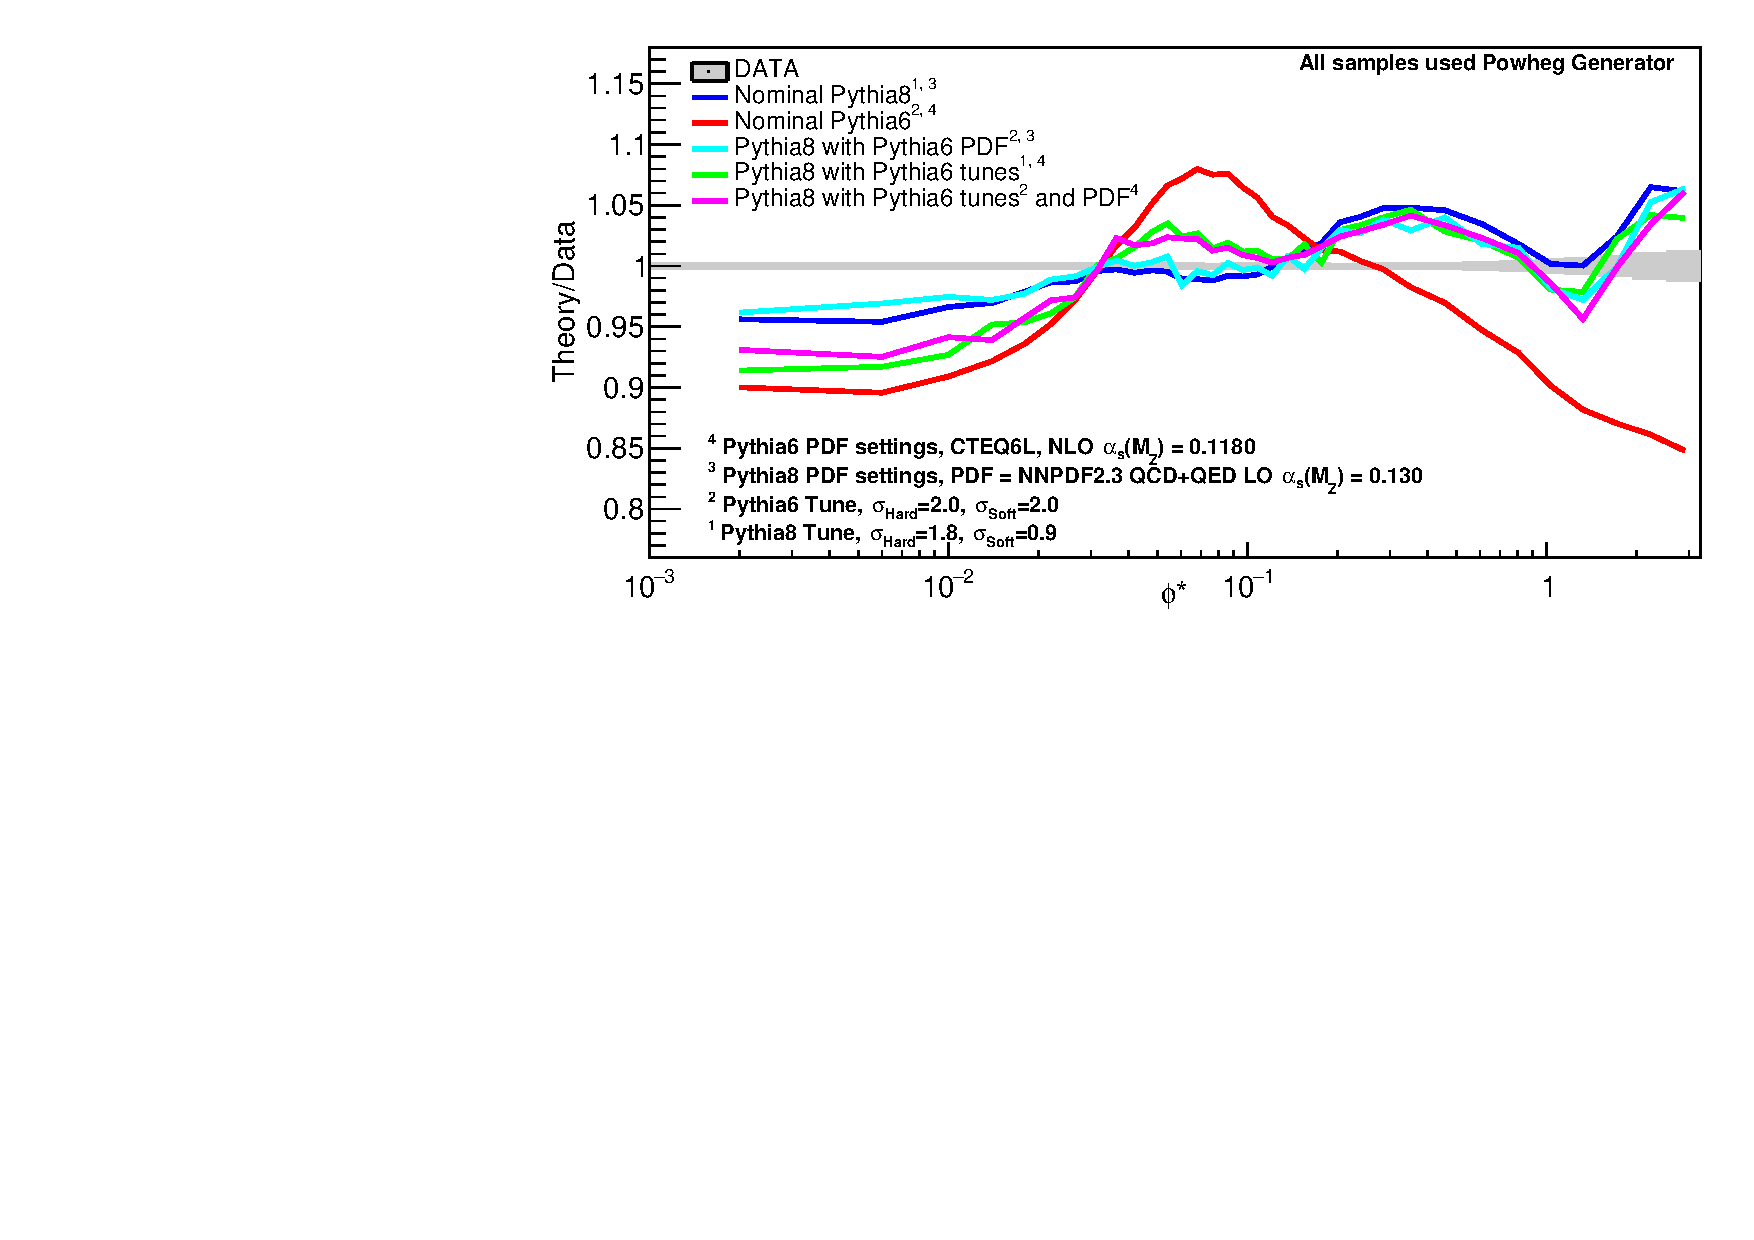
\includegraphics[width=1.1\textwidth]{figures/AnalysisSection/LineLONGRatioComparisonsFinal.pdf}
    \caption[\PYTHIAeight with \PYTHIAsix settings]{When \PYTHIAeight settings were changed to settings used to create the \PYTHIAsix sample, \PYTHIAeight gained some characteristics of the \PYTHIAsix generated sample. These include a very noticeable deficit of events in low \phistar, as well as an excess of events at medium \phistar. However, neither changes to the tune, nor changes to the PDF had much effect at high \phistar  }
    \label{fig:PythiaEightToSix}
\end{figure}{}

\section{Tuning Results}
In order to test the effectiveness of changing \PtWidth to correct the differences between the theory and the data, multiple tunes were tested by changing $\SigmaHard$ and $\SigmaSoft$ independently. As was mentioned last section, lowering \PtWidth, in this case by lowering either $\SigmaSoft$ or $\SigmaHard$, lowered the disagreement in the low \phistar region by  increasing the number of events with low \bosonpt, with four examples shown in Fig.~\ref{fig:AnalysisResult}.It is worth noting that changes to $\SigmaHard$ and $\SigmaSoft$ have nearly the exact same effect on the overall shape of the \phistar distribution since lowering either lowers the \PtWidth of partons produced in the simulation, though by different amounts depending on the energy of the particular gluon involved.


\begin{figure}[!htbp]
    \centering
    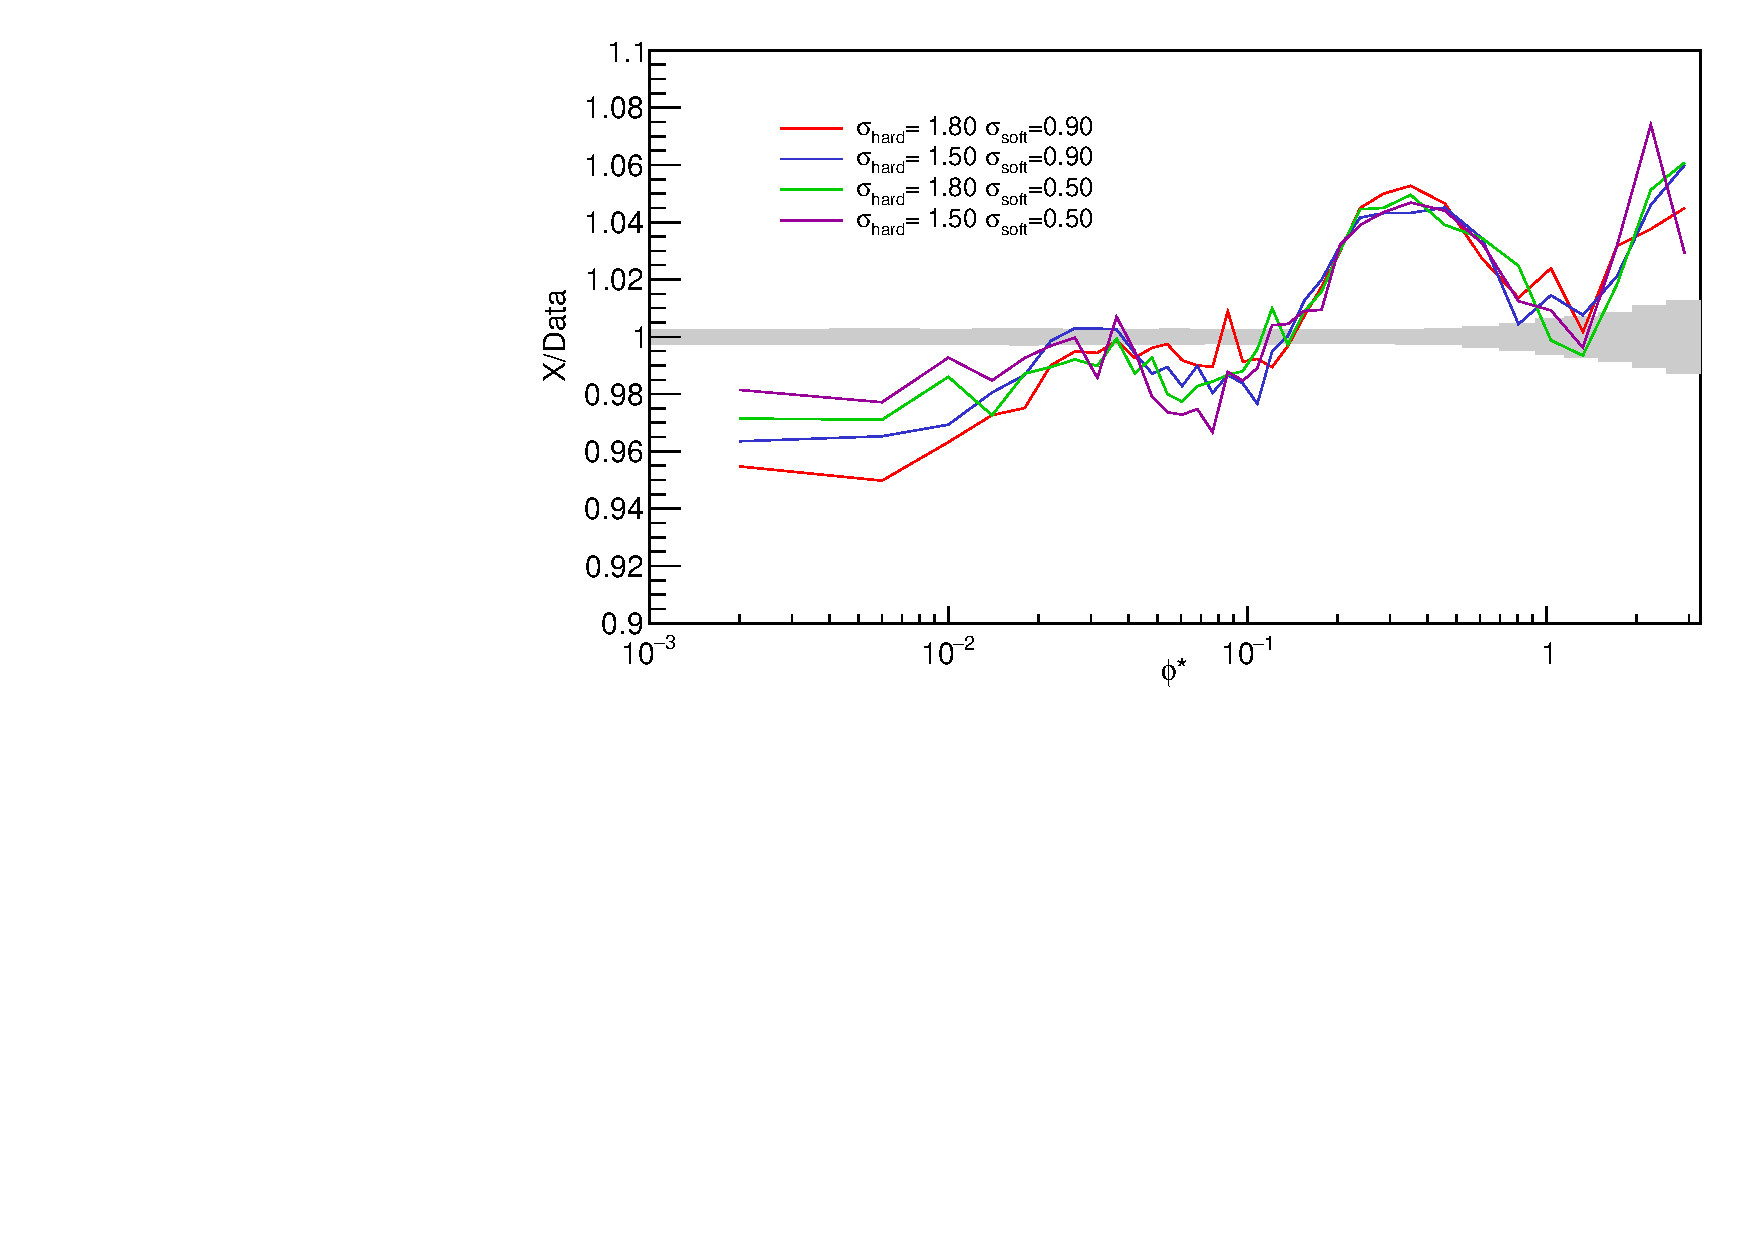
\includegraphics[width=\textwidth]{figures/AnalysisSection/PhistarDistributionsCompareLines.pdf}
    \caption[Data compared with multiple different \POWHEG + \PYTHIAeight distributions]{A plot comparing multiple different tunes to the data. As can be seen there is no tune that provides an improvement in all bins, nor any tune that affects the high \phistar region}
    \label{fig:AnalysisResult}
\end{figure}

Although the changes to $\SigmaHard$ and $\SigmaSoft$ can improve the agreement between simulation and data for low \phistar, the same changes lead to increased disagreement in the mid \phistar and have no noticeable effect on the high \phistar region.  The disagreement in very high \phistar($<1$) is considered acceptable in this study due to the method of which \POWHEG produces events, since it inherently will limit the number of high energy jets produced which can affect the high \bosonpt distribution.  However this explanation does not explain the disagreement of the simulation in the rest of \phistar, which contains the majority of events and is therefore vital to improving the W mass measurement uncertainty.

\subsection{The reweighting of inherent \pt}
In order to compare the effect of different values of \SigmaHard and \SigmaSoft on the \phistar distribution usually multiple simulations would need to be created. The issue with this is it is very resource intensive, both in terms of the scale of computer time to create them as well as having hard drive space to store them. This study would normally require a simulation sample for each combination of \SigmaHard and \SigmaSoft that was compared.  Instead only a couple simulated samples were produced and new \phistar distributions  were created based on other  \SigmaHard and \SigmaSof using a central distribution.

In simulation, \bosonpt is affected by both the generator and the hadronizer used to produce the samples. As was mentioned in Section \ref{sec:HighOrder}, the \px and \py of each parton of the initial state, as well as the particles that were created in their evolution, such as radiated gluons, are chosen using a Gaussian distribution whose width is determined using Eq. \ref{eq:RemWidth}, leading to a probability density function of the form:
\begin{equation}
   G(\px,\py,\PtWidth)=P(\px,\PtWidth)*P(\py,\PtWidth)
\end{equation}{}
\begin{equation}
    =\frac{1}{\sqrt{2\pi}\PtWidth}e^{\frac{-\px^2}{2\PtWidth}}*\frac{1}{\sqrt{2\pi}\PtWidth}e^{\frac{-\py^2}{2\PtWidth^2}}
\end{equation}{}
\begin{equation}
    =\frac{1}{2\pi\PtWidth^2}e^{\frac{-p^{2}_t}{2\PtWidth^2}}.
\end{equation}
Because changes to $\SigmaSoft$ and $\SigmaHard$ do not change any inherent function of the hadronizers, but rather the probability distribution of $\px$ and $\py$, any interaction that happens with one set of values has an easily calculated probability to have happened with a different value of \PtWidth. This allows for the sample to be weighted on an event by event basis to simulate a sample created using different set of tuning parameters. This new event weight is calculated by multiplying the weight due to each separate parton together, $i$,  as shown in: 
\begin{equation}\label{eq:ReW}
W_{event}
=
\prod_i \frac{Prob(\px_i,\py_i,\sigma_{i,new})}{Prob(\px_i,\py_i,\sigma_{i,old})}
=\prod_i \frac{\sigma_{old}^2}{\sigma_{new}^2}e^{\frac{-p_t^2}{2}*(\frac{1}{\sigma_{i,new}^2}-\frac{1}{\sigma_{i,old}^2})}.
\end{equation}
	
This saves a large amount of time and space by not requiring each tune to be created individually. An example demonstrating this reweighting is shown in Fig \ref{fig:Reweighted}, which compares a generated sample using $\SigmaHard=1.5$ to a sample generated using $\SigmaHard=1.8$ that had been reweighted to $\SigmaHard=1.5$ . The reweighted $\SigmaHard=1.8$ matches well to $\SigmaHard=1.5$, with the majority of bin disagreements being near the size of the uncertainty. \par
\begin{figure}[!htb]
    \centering
    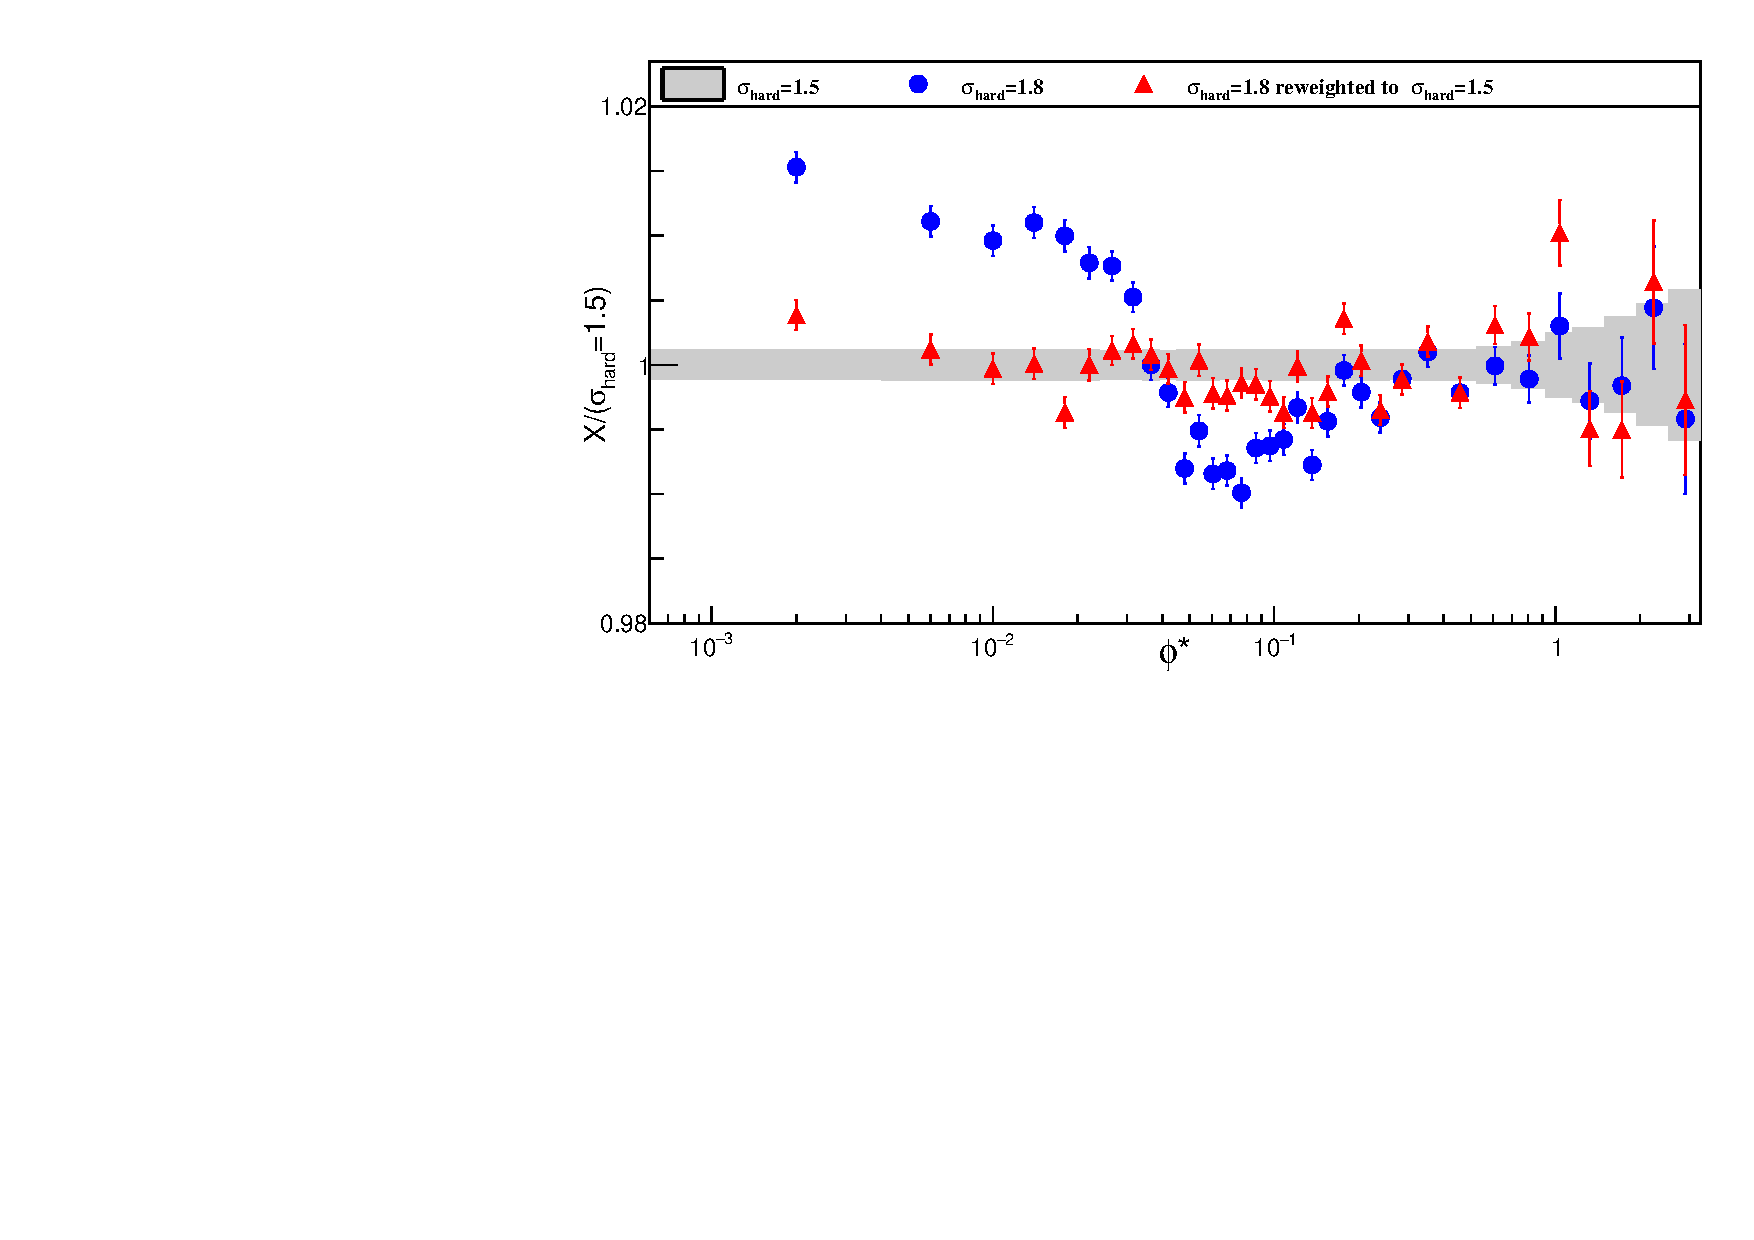
\includegraphics[width=.8\textwidth]{figures/AnalysisSection/RatioRewighted.pdf}
    \caption[Ratio of \phistar Between a specific tune and reweighed tune]{The ratio of a generated \phistar  distribution using $\SigmaHard=1.5$, $\SigmaHard=1.8$, as well at $\SigmaHard=1.8$ that has been reweighted to create a $\SigmaHard=1.5$ distribution. As can be seen, after reweighting $\SigmaHard=1.8$ the distribution fits within 0.5\% of the $\SigmaHard=1.5$ distribution for low \phistar}
    \label{fig:Reweighted}
\end{figure}
However, as the tunes get farther from the central tune that was produced, some weights become extremely large, leading to a larger statistical error. This  limits how far from the central value this method can function effectively. This can be seen in Fig \ref{fig:ReweightedDistribution}, where the events that are far from the central tune ($\SigmaHard=1.8$, $\SigmaSoft=0.9$), the uncertainty increases greatly. Events with similar weights to the central weight have very similar uncertainties. However, due to events with very high weights($>1,000$), the uncertainties grow quickly, increasing by over a factor 10 for most bins of the sample farthest from the central tune. 
	
	\begin{figure}[!htbp]
	    \centering
	    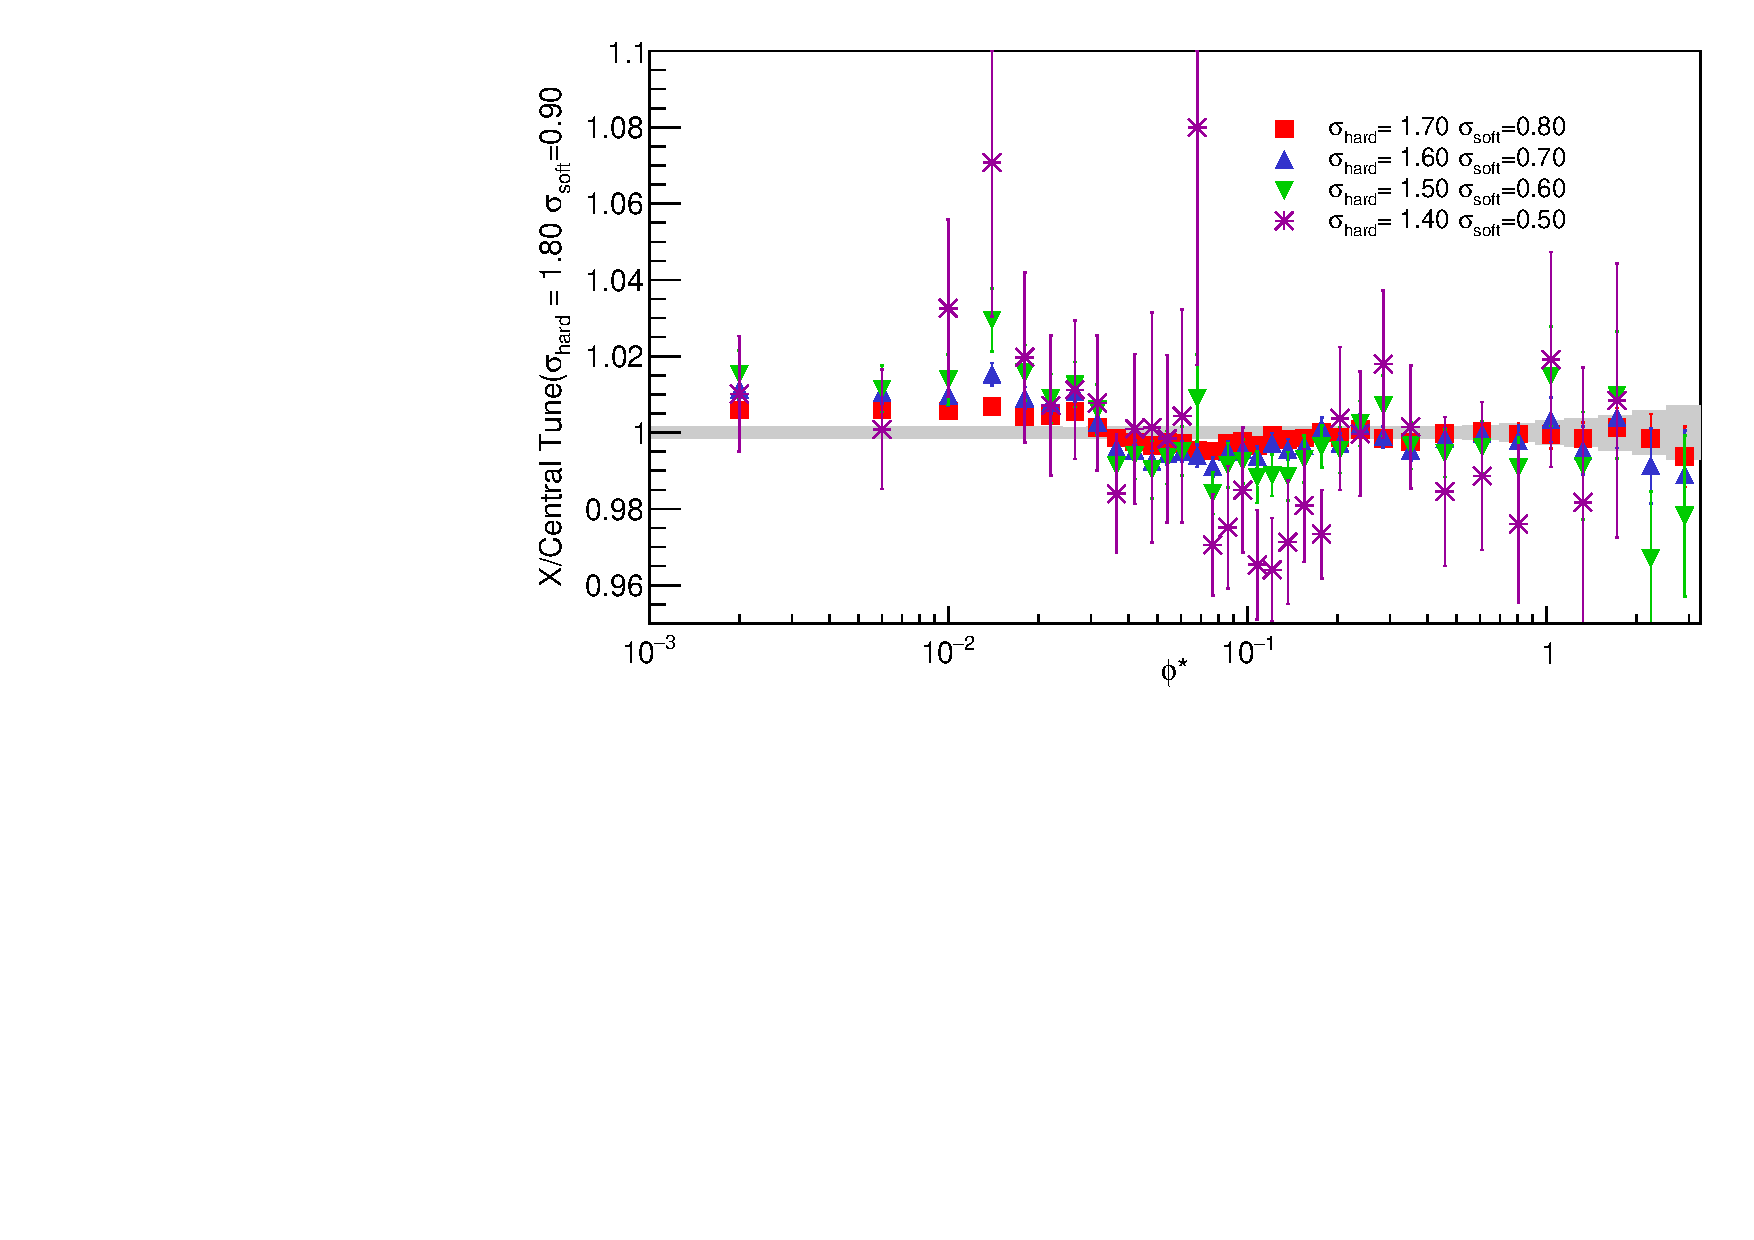
\includegraphics[width=.8\textwidth]{figures/AnalysisSection/PhistarDistributionsTuneOnlyCompare.pdf}
	    \caption[A comparison of retuned distribution]{
	    A plot showing different \phistar distributions over the a central tune. All these distributions are retunes of a single data set with $\SigmaHard=1.8$ and $\SigmaSoft=0.9$. As can be seen for the tunes closest to the central tune have very small statistical fluctuations, but the tunes farthest from the central tune have large fluctuations from bin to bin.
	    }\label{fig:ReweightedDistribution}
	\end{figure}
Figure \ref{fig:PartonWeight} shows the parton weights used when converting from a central tune($\SigmaHard=1.8$ and $\SigmaSoft=0.9$), to others. As the tunes get further from the central tune, the peak widens and moves to a larger value, though all distributions drop quickly after the peak. These weights are relatively small, with no events with weights larger than 3.
	
	\begin{figure}[!htb]
	    \centering
	    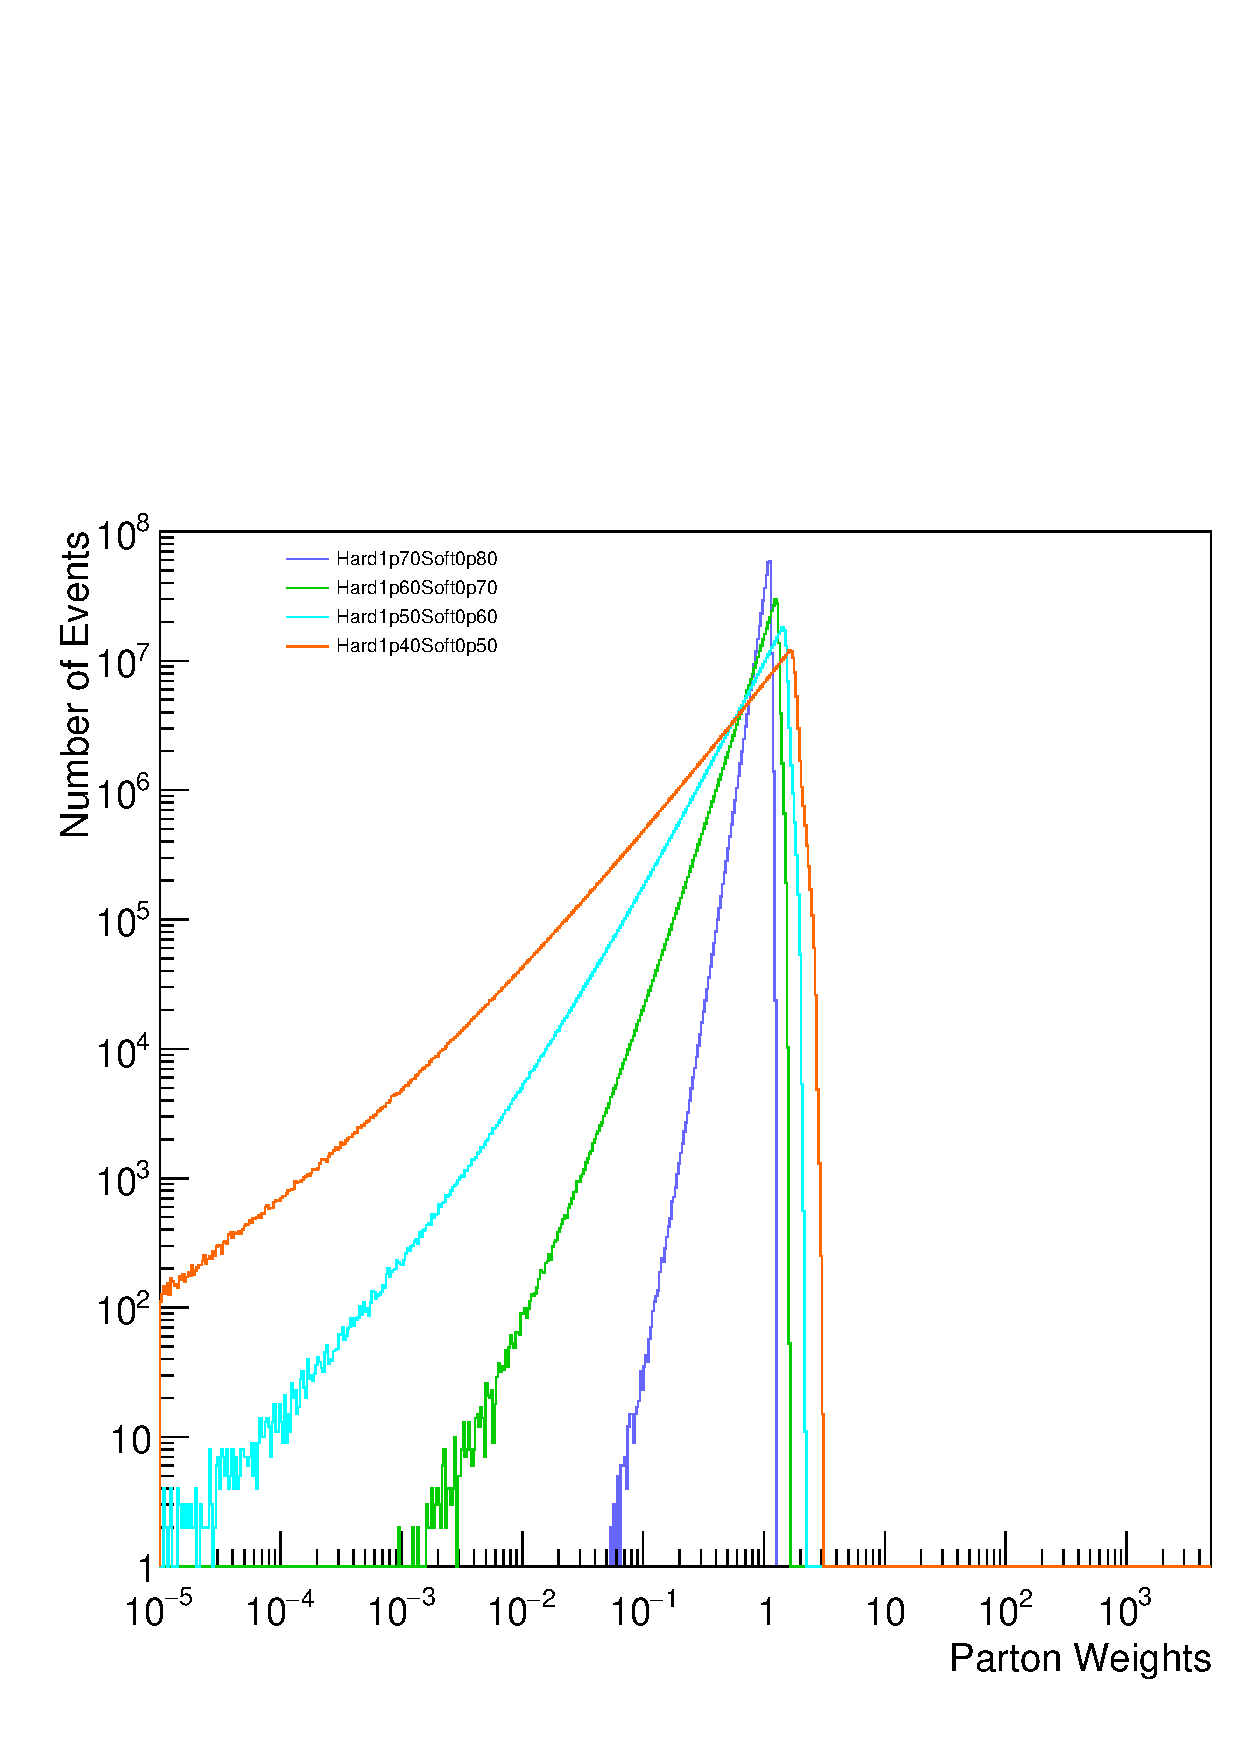
\includegraphics[width=.9\textwidth]{figures/AnalysisSection/PartonWeights.pdf}
	    \caption[Parton Weights]{ Although many of the partons weights are $<1$, there are almost no partons with weights more than a factor of 3.}
	    \label{fig:PartonWeight}
	\end{figure}
	Despite these small weights, due to the multiplicative nature of the weights of each parton, the total weight covers a wide range of possible values, as shown in Fig. \ref{fig:EventWeights}. As is demonstrated by $\SigmaHard=1.4$ and $\SigmaSoft=0.5$, when a sample is changed to a drastically different tune weights can become extremely large, with some events of having weights of the order of ten thousand. Because all bins, excluding the high \phistar tail, contain $\approx$ four hundred thousand events, each of these high weighted events can change the binned value by a couple of percentage points, leading to an unacceptably high fluctuation of the bin value. To remove this issue, this reweighting method is limited to changing the tune by requiring  that:
	\begin{equation}
	    0.25>\sqrt{\left(\frac{\SigmaHard^*-\SigmaHard}{\SigmaHard}\right)^2+\left(\frac{\SigmaSoft^*-\SigmaSoft}{\SigmaSoft}\right)^2}.
	\end{equation}{}
	\begin{figure}[!htb]
	    \centering
	    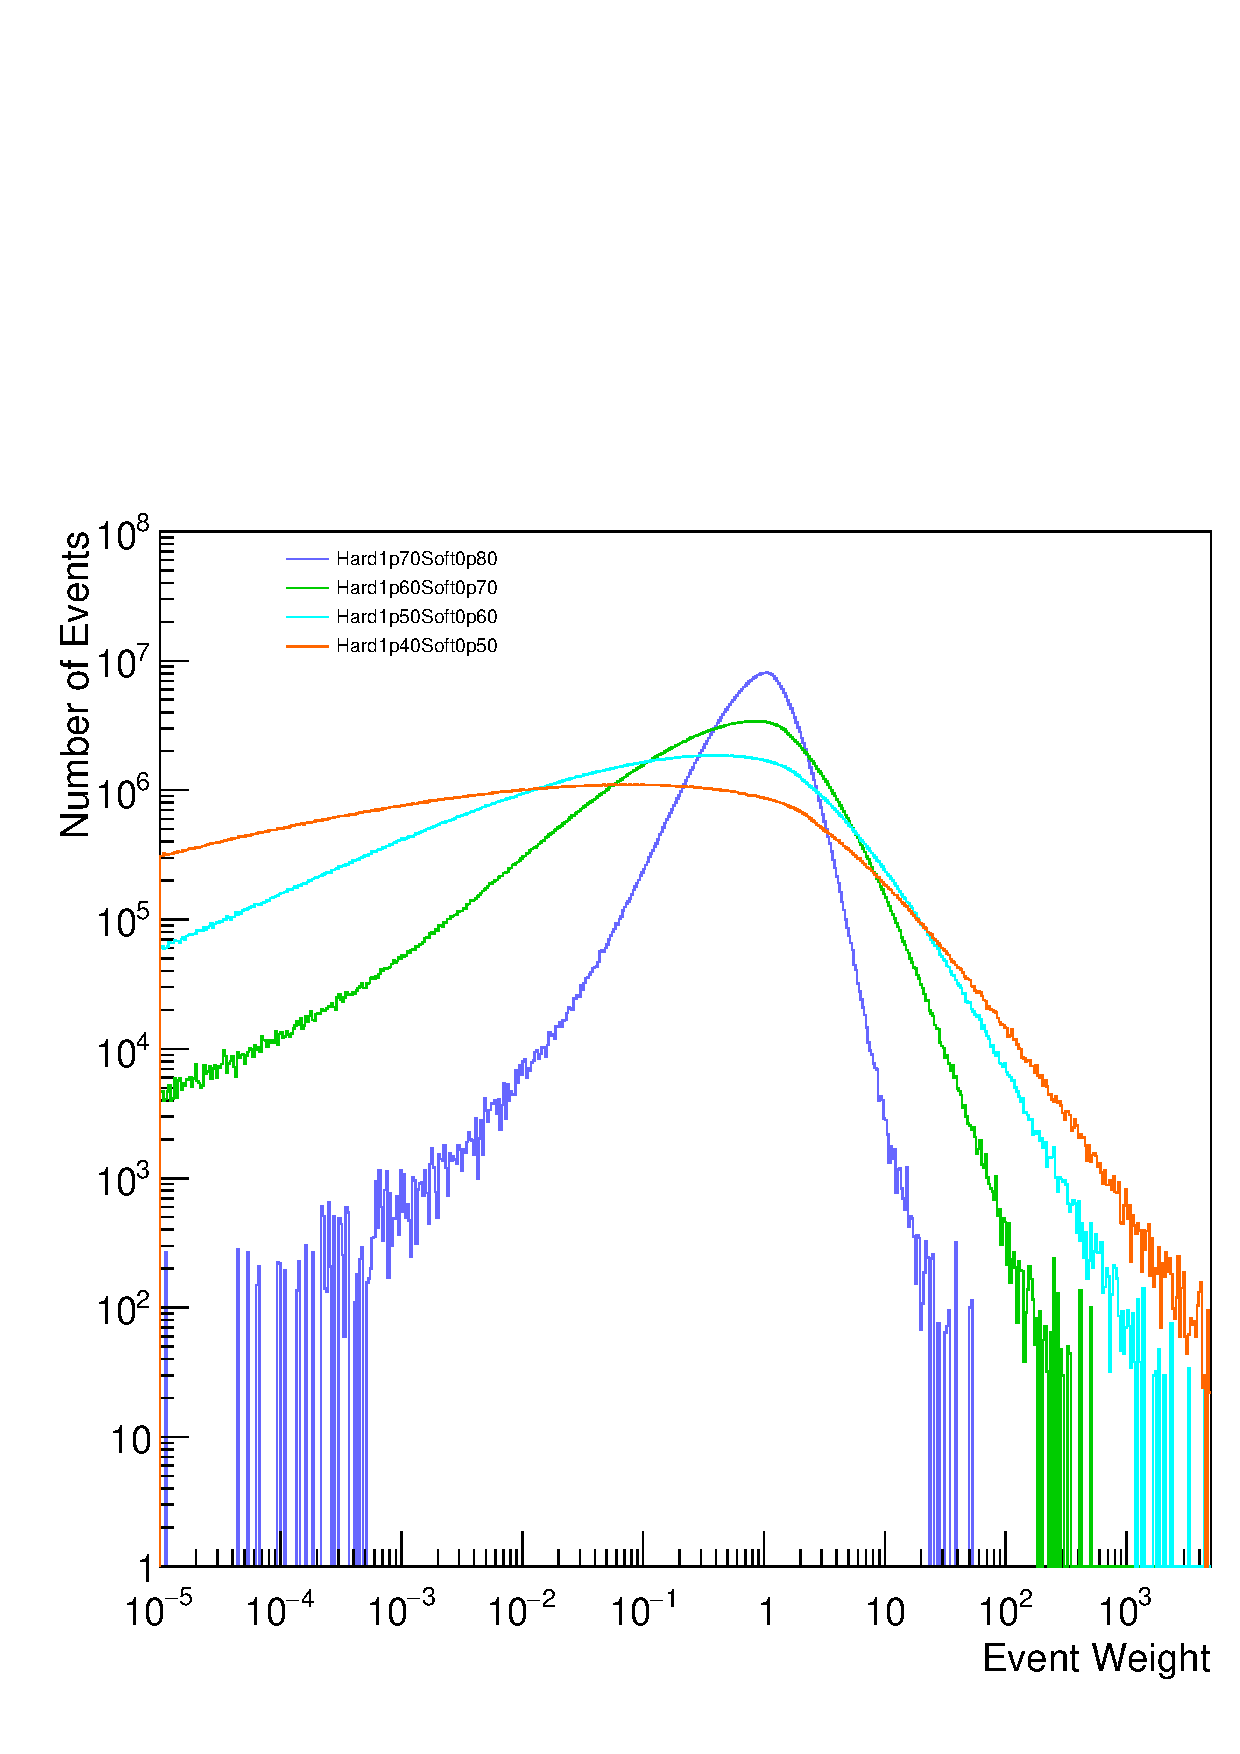
\includegraphics[width=.8\textwidth]{figures/AnalysisSection/TotalEventWeights.pdf}
	    \caption[Event weights]{Event weights for changing the tunes. As can be seen as the tune gets further from the central tune of $\SigmaHard=1.8$ and $\SigmaSoft=0.9$, the distributions get wider, with the  $\SigmaHard=1.4$ and $\SigmaSoft=0.5$ having multiple events of the order of 10,000.}
	    \label{fig:EventWeights}
	\end{figure}
	
	Despite limitations of this reweighting, being unable to drastically change \SigmaHard and \SigmaSoft, this reweighting method allows for distributions to be created fast and efficiently using a central distribution.   
%%%%%%%%%%%%%%%%%%%%%%%%%%%%%%%%%%%%%%%%%%%%%%%%%%%%%%%%%%%%%%%%%%%%%%%%%%%%%%%%
\label{neymanana}

%%%%%%%%%%%%%%%%%%%%%%%%%%%%%%%%%%%%%%%%%%%%%%%%%%%%%%%%%%%%%%%%%%%%%%%%%%%%%}}}
